\documentclass{book}
\usepackage{mathalpha}
\usepackage[utf8]{inputenc}
\usepackage{cancel}
\usepackage[margin=2cm, a4paper]{geometry}
\usepackage{amsmath}
\usepackage{amssymb}
\usepackage{gensymb}
\usepackage{graphicx}
\usepackage{hyperref}
\usepackage{pgfplots}
\usepackage{tikz}
\usepackage{pdfpages}
\usepackage{parskip}
\usepackage{polynom}
\usepackage{multirow}

\title{Chemistry}
\author{Lachlan Takumi Ikeguchi}

\begin{document}
\maketitle
\tableofcontents

\section{The purpose}
This document was written to be used as a summary to help revise the content covered in Chemistry.  For any inquiries, feedback, and further explanations, contact lachlanprivate@duck.com or through the discord server: \url{https://discord.gg/6P8rddkXFr}.  I encourage you to let me know of any topic I missed, how I could explain it better, or how it could be reworded or formatted to be more helpful in its purpose.  The goal of this document is to be a comprehensive summary of everything you need to know.

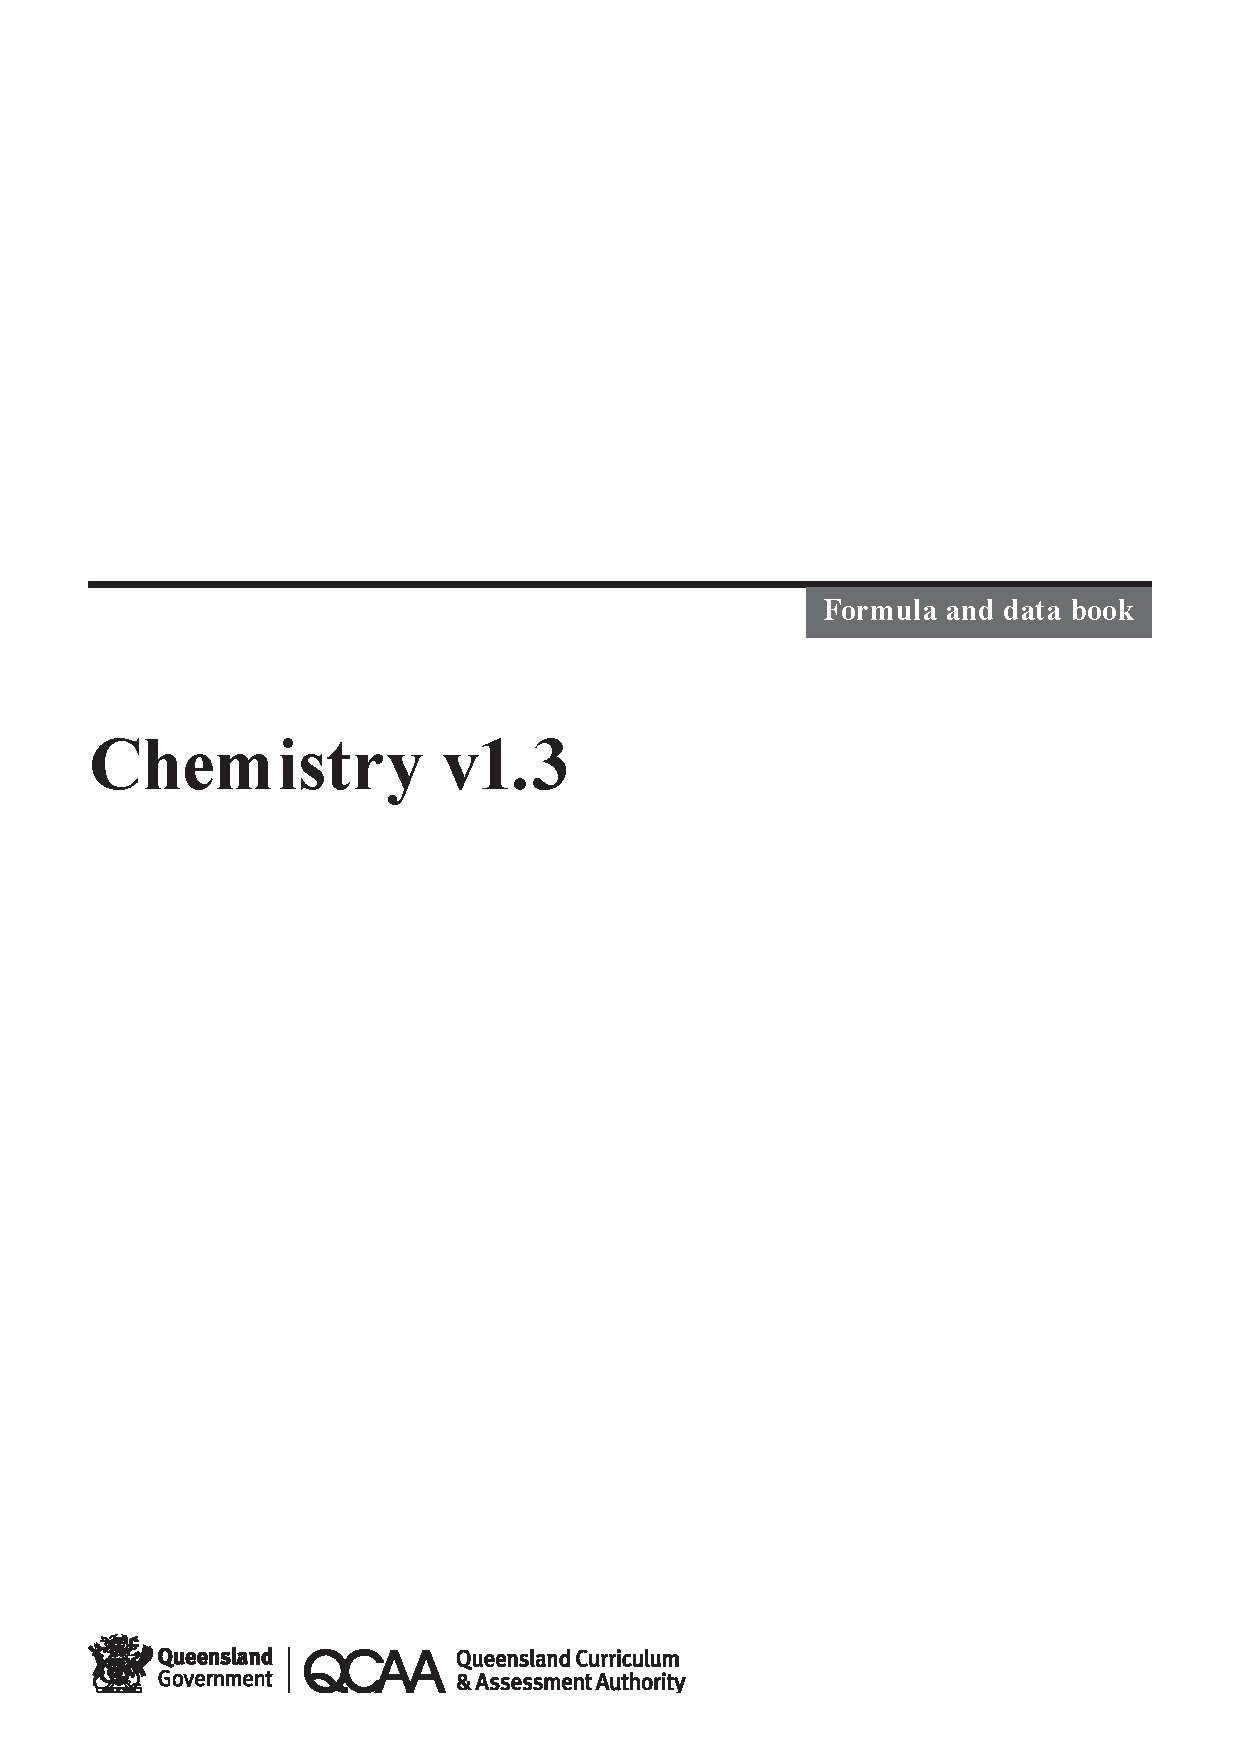
\includepdf[pages={1-16}]{./images/formula-book.pdf}

\chapter{Atomic structures}

\chapter{Periodic table and trends}

\chapter{Electron configurations}

\chapter{Atomic absorption spectroscopy}

\chapter{Isotopes}

\chapter{Mass spectroscopy}

\chapter{Bonding}
\section{Ionic}

\section{Covalent}

\section{Polyatomic}

\chapter{Lewis structures}

\chapter{Properties}
\section{Elements}

\section{Compounds}

\section{Mixtures}

\chapter{Organic chemistry}

\chapter{Nanomaterials}

\chapter{Reactions}
\section{States of matter}

\section{Balancing equations}

\section{Types of reactions}

\section{Enthalpy}

\section{Specific heat capacity}

\section{Mole concept}

\section{Limiting reagents}

\section{Emperical formula}




\end{document}